\chapter{Robôs Móveis}
\label{robosMoveis}

  Neste capitulo serão discutidas algumas das principais tarefas que o robô deve desempenhar,
  para que ele possa concluir seu objetivos de forma autônoma e da melhor maneira possível, sendo elas: localização e construção de mapas.
  
\section{Localização}
A obtenção da posição e orientação(pose) do robô pode ser feita através da identificação e 
subsequente triangulação por ângulos e por distância dos \textit{landmarks} percebidos pelo robô e
 previamente conhecidos. Onde a identificação dos \textit{landmarks} 
 é feita fazendo observações do ambiente utilizando seus sensores(sonar, laser, câmera).
 
 No calculo da localização o robô deve ser capaz de lidar com os erros de medição dos sensores, 
 incertezas(que tendem a crescer com o deslocamento do robô) 
 e informações incompletas \cite{localization1}.  Portanto, ao invés de calcular a posição exata, 
 o que pode ser feito é calcular a probabilidade do robô estar numa certa posição. Daí a necessidade da 
 localização probabilística, na qual, a incerteza é representada utilizando teoria da probabilidade: 
 ao invés de dar a melhor estimativa da configuração atual do robô, 
 a localização probabilística nos da a distribuição de probabilidade de todas as possíveis 
 configurações do robô \cite{localization1}. Essa distribuição de probabilidade é chamada \textit{belief}.
 
 Quando o robô se movimenta a incerteza de sua posição aumenta. 
 Fazendo observações do ambiente e mesclando os dados obtidos com a estimação da odometria, 
 o robô pode combinar essas informações com o \textit{belief} anterior ao deslocamento. 
 Deste modo, a cada movimento o robô pode
 obter uma melhor estimativa de sua real posição, isso é chamado modelo de movimento e percepção.
 
 A cada deslocamento do robô é necessário fazer a atualização da distribuição de probabilidade de sua configuração, 
 a atualização pode ser dividida em 2 passos \cite{localization1}:
 \begin{itemize}
  \item Atualização de ação: o robô se move e estima sua posição através de seus sensores nesse passo a incerteza aumenta.
  \item Atualização de percepção: o robô faz uma observação usando seus sensores e corrige sua posição, 
  combinando seu \textit{belief} com a probabilidade de fazer essa observação.
  Aqui a incerteza diminui.
 \end{itemize}

 No calculo da localização probabilística é necessário ter: a distribuição de probabilidade inicial, 
 o modelo de erro estatístico dos sensores e o mapa do ambiente.
 Há duas principais abordagens para solução da localização probabilística de robôs móveis: 
 localização de Markov e filtro de Kalman, descritos a seguir.  
 
 \subsection{Localização de Markov}
	A localização de Markov usa um \textit{grid} para representar a configuração do robô, onde cada célula do \textit{grid}
	contêm a probabilidade de robô estar nela \cite{localization1}. A distribuição de probabilidade associada à percepção 
	dos sensores também é discretizado. Durante as etapas de ação e percepção todas as células do \textit{grid} são atualizadas. 
	
	A atualização na etapa de ação é feita através da convolução da distribuição do \textit{belief} inicial com a distribuição
	da probabilidade da possível pose do robô após seu deslocamento, com a incerteza aumentada, segundo o modelo de deslocamento.
	Na etapa da percepção, a atualização e feita fazendo a convolução do \textit{belief} inicial com o modelo estatístico de erro
	dos sensores. A convolução pode ser feita através da regra de Bayes\cite{localization1}.
	
	A ideia principal da regra de Bayes é que a probabilidade de um evento A dado um evento B 
	depende não apenas do relacionamento entre os eventos A e B, 
	mas também da probabilidade marginal (ou "probabilidade simples") da ocorrência de cada evento:
	
	\begin{figure}[hb]
	\centering
	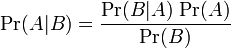
\includegraphics[scale=0.7]{images/bayes.png}
	\caption{Regra de Bayes.}
	\label{fig:topologia}
	\end{figure}
	
	Como todas as células são atualizadas nas etapas de ação e percepção, a localização de Markov requer grande 
	quantidade de processamento e memória.
 
 \subsection{Localização filtro de Kalman}
 
 
 Na localização filtro de Kalman, assume-se que a distribuição de probabilidade da configuração do robô e o modelo dos sensores,
 são continuas e gaussiana \cite{localization2}. Como a distribuição gaussiana é descrita através da média e variância, somente essas duas variáveis 
 são atualizadas nas etapas de ação e percepção. Portanto, seu custo computacional é pequeno se comparado com a localização de Markov.
 
O filtro de Kalman produz estimativas dos valores reais de grandezas medidas e valores associados predizendo um valor, 
estimando a incerteza do valor predito e calculando uma média ponderada entre o valor predito e o valor medido. 
O peso maior é dado ao valor de menor incerteza. As estimativas geradas pelo método tendem a estar mais próximas dos 
valores reais que as medidas originais pois a média ponderada apresenta uma melhor estimativa de incerteza que ambos os valores utilizados no seu cálculo.

 %inferências exatas sobre um sistema dinâmico linear, mas onde o espaço de estados das variáveis não observadas é contínuo e todas as variáveis, observadas e não observadas, apresentam distribuição normal (ou, frequentemente, distribuição normal multivariada).
 
  %A estimativa obtida desta forma é melhor que a estimativa obtida utilizando-se qualquer uma das medidas unicamente. Assim, é um algoritmo usual para fusão de sensores.
%Na execução dos cálculos para o filtro, a estimativa do estado e as covariâncias são representadas por matrizes,
%para tratar as múltiplas dimensões envolvidas num único passo do cálculo. 
%Desta forma, é possível representar as relações lineares entre diferentes variáveis de 
%estado (como posição, velocidade e aceleração) em qualquer um dos modelos de transição ou covariâncias, 
%onde o espaço de estados das variáveis apresentam distribuição normal.
  
O filtro de Kalman combina uma predição da posição atual do robô a com uma nova medida usando uma média ponderada. 
A ideia dos pesos é que valores com menor incerteza estimada sejam mais "confiáveis". 
Os pesos são calculados através da covariância, uma medida da incerteza estimada da predição do estado do sistema. 

O resultado da média ponderada é uma nova estimativa do estado, que se localiza entre o estado predito e o estado medido, 
apresentando uma melhor incerteza estimada que qualquer um dos dois unicamente. 
Este processo é repetido a cada fase, com a nova estimativa e sua covariância gerando a predição usada na próxima iteração. 
Isto significa que o filtro de Kalman funciona recursivamente e requer apenas a 
última estimativa - não o histórico completo - do estado de um sistema para calcular o próximo estado.

 
 \begin{comment}
  The probability distribution of both the
robot configuration and the sensor model is
assumed to be continuous and
Gaussian!
• Since a Gaussian distribution only
described through mean value
μ
and
variance
σ
2
, we need only to update
μ
and
Σ
2.
Therefore the computational cost is
very low!

 Localization is tracked from a known positions
and recovery from ambiguous situations and after
collision is not possible
\end{comment}


\section{Construção de Mapas}
A tarefa de mapeamento corresponde à atribuição de valores aos elementos do mapa, relacionando cada um a uma certa 
posição nele \cite{construcaoMapas2}. O tipo ideal de mapa
a ser utilizado ou construído por um robô móvel depende da tarefa e do ambiente onde
este esteja inserido. Também depende das características do robô, tais como os tipos
de sensores que ele tem, bem como a forma com ele se move\cite{construcaoMapas2}.  Há duas abordagens principais para a 
representação de mapas de ambiente \cite{construcaoMapas}.
São os mapas métricos e topológicos, que serão discutidos a seguir. 

\subsection{Mapas Métricos}
No caso da construção de mapas métricos, o objetivo é obter um mapa detalhado do ambiente, 
com informações sobre a forma e o tamanho dos objetos e os limites das
áreas livres para a navegação, tais como corredores, quartos, trilhas e estradas. Para
representar essa complexa e detalhada informação, o mapa é geralmente dividido em
uma densa rede de forma que cada célula contenha informações sobre a ocupação
desse espaço por um objeto e, possivelmente, outras características ambientais que
estão sendo mapeadas \cite{construcaoMapas2}. 

Com à alta densidade de informação nesses mapas, o resultado da localização é mais preciso e
menos sujeito a ambiguidades \cite{construcaoMapas2}. Como os mapas métricos 
demandam uma grande quantidade de informações, eles exigem muita capacidade de processamento e 
armazenamento.

Atualmente grande parte dos sistemas de mapeamento assumem que o ambiente é estático
durante o mapeamento. Se uma pessoa anda dentro do alcance dos sensores do robô durante o
mapeamento, o mapa resultante conterá evidências a respeito de um objeto na localização
correspondente. Além disso, se o robô retornar para esta localização e varrer a área uma
segunda vez, sem a pessoa presente, a estimativa da posição será menos precisa, uma vez que as novas medições não
contêm nenhum vestígio correspondente àquela pessoa. A exatidão reduzida do mapa
resultante pode ter uma influência negativa no desempenho da localização robô.

\subsection{Mapas Topológicos}
No caso de mapas topológicos, o objetivo é construir uma estrutura relacional, normalmente um grafo, 
de forma geral, registram informações sobre determinados
elementos ou locais do ambiente, chamados marcos \cite{construcaoMapas2}. 
Assim, marcos e relações são os elementos dos mapas topológicos.
Essas relações podem ser de vários tipos, tais como o deslocamento
relativo entre dois marcos, a existência de um caminho entre eles,
quantidade de energia gasto em um caminho entre marcos,etc. 
É fácil perceber que a informação contida no mapa topológico é
menos detalhada e distribui-se de forma dispersa, concentrando-se apenas em pontos de interesse.
Assim esta representação, é muito seletiva com relação à informação que ele registra \cite{construcaoMapas2}. 

O mapa topológico também demanda que o processamento
dos dados dos sensores do robô, sejam feitos de forma mais abstrata, 
a fim de extrair informações sobre as localidades mais relevantes que devem ser consideradas
como marcos.

\section{Problema de auto localização e mapeamento simultâneos}
  O problema de auto localização e construção de mapas de ambiente simultâneos (\textit{Simultaneous Localization and
Map Building - SLAM}) consiste em um robô autônomo iniciar a navegação
em uma localização desconhecida, em um ambiente desconhecido e então construir um mapa
desse ambiente de maneira incremental, enquanto utiliza o mapa simultaneamente para calcular a sua localização \cite{slam}.
 
 O SLAM tem sido tema de várias pesquisas na área de robótica. A grande vantagem do SLAM é que elimina a necessidade 
um conhecimento topológico a priori do ambiente. Há três abordagens principais que são utilizadas no problema do SLAM. 
\begin{comment}
Pick natural scene features to serve as landmarks
(in most modern SLAM systems)

Range sensing (laser/sonar): line segments, 3D planes, corners

Vision: point features, lines, textured surfaces.

Key
: features must be distinctive & recognizable from different viewpoints

Keeping track of
changes in the environmen

Map can become inconsistent due to
erroneous measurements / motion drift

Their position uncertainty results
from the combination of the
measurement error with the
robot
pose
uncertainty


map becomes correlated with
the robot
pose
estimate

Robot moves again and its
uncertainty increases
(
motion
model)

Robot re
-
observes an old feature

Robot updates its position: the
resulting position estimate
becomes correlated with the
feature location estimates.

Robot‟s uncertainty shrinks and so
does the uncertainty in the rest of
the map
\end{comment}

A primeira e mais popular deles usa o filtro de Kalman estendido para resolver o SLAM(Extended Kalman Filter SLAM - EKF SLAM) \cite{slam2}. Ele
fornece uma solução recursiva para o problema da navegação e uma maneira de calcular
estimativas consistentes para a incerteza na localização do robô e nas posições dos marcos do
ambiente, com base em modelos estatísticos para o movimento dos robôs e observações
relativas dos marcos do ambiente\cite{slam}.

O EKF SLAM resume toda a toda experiencia obtida pelo robô em um vetor de estados estendido $Y$, compreendendo a pose do 
robô, a posição dos marcos do mapa e a matriz de covariância $P$\cite{slam2}. Quando o robô se desloca $Y$ e $P$ são atualizadas
usando o EKF. Os marcos do ambiente são extraídos do ambiente de sua nova posição. Em seguida, o robô tenta associar esses
marcos com os marcos previamente observados. A Reobservação dos marcos são usados para atualizar a posição do robô. 
Os marcos que não foram observados previamente, são adicionados no mapa de marcos.

\begin{comment}
When the odometry changes because the robot moves t
he uncertainty pertaining to the
robots new position is updated in the EKF using Odo
metry update. Landmarks are
then extracted from the environment from the robots
new position. The robot then
attempts to associate these landmarks to observatio
ns of landmarks it previously has
seen. Re-observed landmarks are then used to updat
e the robots position in the EKF.
Landmarks which have not previously been seen are a
dded to the EKF as new
observations so they can be re-observed later. All
these steps will be explained in the
next chapters in a very practical fashion relative
to how our ER1 robot was
implemented. It should be noted that at any point
in these steps the EKF will have an
estimate of the robots current position. 

Landmarks are features which can easily be re-obser
ved and distinguished from the
environment. These are used by the robot to find o
ut where it is (to localize itself).
One way to imagine how this works for the robot is
to picture yourself blindfolded. If
you move around blindfolded in a house you may reac
h out and touch objects or hug
walls so that you don’t get lost. Characteristic t
hings such as that felt by touching a
doorframe may help you in establishing an estimate
of where you are. Sonars and
laser scanners are a robots feeling of touch. 

Landmarks should be re-observable by allowing them
for example to be viewed
(detected) from different positions and thus from d
ifferent angles.
Landmarks should be unique enough so that they can
be easily identified from one
time-step to another without mixing them up. In ot
her words if you re-observe two
landmarks at a later point in time it should be eas
y to determine which of the
landmarks is which of the landmarks we have previou
sly seen. If two landmarks are
very close to each other this may be hard

The key points about suitable landmarks are as foll
ows:
Landmarks should be easily re-observable.
Individual landmarks should be distinguishable from
each other.
Landmarks should be plentiful in the environment.
Landmarks should be stationary. 

The first step is very easy. It is just an addition
of the controls of the robot to the old
state estimate. E.g. the robot is at point (x, y) w
ith rotation theta and the controls are
(dx, dy) and change in rotation is dtheta. The resu
lt of the first step is the new state of
the robot (x+dx, y+dy) with rotation theta+dtheta.
In the second step the re-observed landmarks are co
nsidered. Using the estimate of the
current position it is possible to estimate where t
he landmark should be. There is
usually some difference, this is called the innovat
ion. So the innovation is basically
the difference between the estimated robot position
and the actual robot position,
based on what the robot is able to see. In the seco
nd step the uncertainty of each
observed landmark is also updated to reflect recent
changes. An example could be if
the uncertainty of the current landmark position is
very little. Re-observing a
landmark from this position with low uncertainty wi
ll increase the landmark certainty,
i.e. the variance of the landmark with respect to t
he current position of the robot.
In the third step new landmarks are added to the st
ate, the robot map of the world.
This is done using information about the current po
sition and adding information
about the relation between the new landmark and the
old landmarks. 

http://ocw.mit.edu/courses/aeronautics-and-astronautics/16-412j-cognitive-robotics-spring-2005/projects/1aslam_blas_repo.pdf
http://www.asl.ethz.ch/education/master/mobile_robotics/year2012/Lecture10.pdf
\end{comment}

A segunda abordagem chamada filtro de partículas SLAM, consiste em evitar a necessidade de estimativas absolutas da
posição e de medições precisas das incertezas para utilizar conhecimento mais qualitativo da
localização relativa dos marcos do ambiente e do robô para a construção do mapa global e
planejamento da trajetória\cite{construcaoMapas}. 

O filtro de partículas é um modelo matemático que representa a distribuição de probabilidade associada a um conjunto 
de partículas discretas. Uma partícula contém a estimativa da pose do robô com pesos associados(todos os pesos 
devem ser incrementados em 1) \cite{slam2}. Por período de amostragem, cada partícula é modificada de acordo com o
modelo do processo, incluindo a adição de ruído aleatório para simular o efeito do ruído
nas variáveis de estado e, então, o peso de cada partícula é reavaliado com base na última
informação sensorial. 

As partículas com pesos próximos de zero são descartadas e recriam-se novas partículas com base naquelas que sobram. Quando o
número efetivo de amostras está abaixo de um determinado limiar, geralmente calculado
com base em uma percentagem das M partículas, então a população das M partículas é
re-amostrada (resampling), eliminado-se probabilisticamente aquelas cujos pesos são pequenos
e duplicando aquelas com pesos elevados \cite{slam4}.

\begin{comment}
Particle filters:
mathematical models that represent probability distributions as a
set of discrete particles which occupy the state space.
Particle
= a point estimate of the state with an associated weight
(all weights should add up to 1)

Steps in Particle Filtering:

Predict
:
Apply motion prediction to each particle

Make measurements

Update
:
for each particle:
•
Compare the particle‟s predictions of measurements with the actual measurements
•
Assign weights such that particles with good predictions have higher weight

Normalize
weights of particles to add up to 1

Resample
: generate a new set of M particles which all have equal weights 1/M
reflecting the probability density of the last particle set.

FastSLAM
approach
[
Montemerlo
et al., 2002]
•
Solve state posterior using a
Rao
-
Blackwellized
Particle Filter
•
Each landmark estimate is represented by a 2x2 EKF.
•
Each particle is “independent” (due the factorization) from the others and
maintains the estimate of M landmark positions.
\end{comment}

O terceiro método é bastante amplo e afasta-se do rigor matemático do filtro de
Kalman, ou do formalismo estatístico, retendo uma abordagem essencialmente numérica ou
computacional para a navegação e para o problema de SLAM. Essa abordagem inclui o uso
de correspondência com marcos artificiais do ambiente\cite{construcaoMapas}, ela é chamada de GraphSLAM.
As posições do robô ao longo do tempo e os marcos correspondem a nós em um grafo \cite{slam2}. 
As informações odométricas entre posições consecutivas e os marcos vistos em diferentes posições equivalem as arestas do
grafo. O algoritmo é executado em 2 etapas. Na primeira etapa, o mesmo apenas acumula dados e
constrói o grafo. Na segunda etapa, o o grafo é rearranjado para acomodar
os dados obtidos. Diferente do EKF SLAM, o GraphSLAM estima a posição do robô durante todo o trajeto.

\begin{comment}
GraphSLAM
basic idea: SLAM can be interpreted as a sparse graph of nodes and constraints
between nodes

nodes:
robot locations and map
-
feature locations

edges:
constraints between
consecutive robot poses (given by the
odometry
input
u
) and
robot poses and the features
observed
from
these
poses
.

Key property: constraints are not to be thought as rigid constraints but as soft constraints
constraints acting like
springs

Solve full SLAM by relaxing these constraints
get the best estimate of the robot path and
the environment map by computing the
state of minimal energy
of this network

the
update
-
time
is
constant
and
the required
memory
is
linear
with the no. features
\end{comment}

\begin{comment}
\subsection{Problema de navegação e mapeamento completo do ambiente}
  No artigo \cite{cnn} - \textit{"A Bioinspired Neural Network for Real-Time Concurrent Map Building and Complete Coverage Robot Navigation in Unknown Environments"},
Luo e Yang propõem um modelo de mapeamento e navegação de robôs em ambientes desconhecidos e dinâmicos. Eles utilizam robôs limpadores para exemplificar o modelo. No 
qual o robô deve percorrer todo o local, para fazer sua limpeza.

  O mapa topológico do ambiente é discretizado em células, onde as células podem assumir o formato de quadrados, retângulos e triângulos. 
Utilizando quadrados e retângulos, o robô limpador têm 8 direções possíveis para deslocamento, enquanto que utilizando células triangulares, 
o robô possui 12 direções possíveis, assim permitindo que o robô navegue por caminhos mais curtos e flexíveis. 
Essas células formam uma rede neural, e cada célula pode assumir um estado: desconhecido, limpo, sujo e \textit{deadlock}. 

O mapeamento do ambiente é feito com o robô limpador percorrendo o ambiente em "ziguezague" e monitorando a atividade neural da rede.
A dinamicidade da atividade neural, representa as mudanças do ambiente. As areas sujas e com com obstáculos ficam no topo e no vale da atividade da rede neural, 
respectivamente. As áreas sujas atraem o robô, através da propagação da atividade neural. 
O planejamento do caminho para evitar colisões é feito em tempo real, baseado na dinamicidade da atividade neural da rede e na posição anterior do robô, assim ele 
é capaz de percorrer o ambiente, limpando as áreas sujas.
\end{comment}

\begin{comment}
\section{Planejamento de trajetos}
  O problema planejamento de trajetos, consiste em encontrar o melhor trajeto possível, 
  de um ponto de origem até um ponto de destino que não resulte em colisão com obstáculos \cite{voronoi}.
  Dependendo da quantidade de informação disponível sobre o ambiente, que pode ser completamente ou
   parcialmente conhecido ou desconhecido, as abordagens de planejamento podem variar consideravelmente.
   A definição de melhor trajeto também pode variar. Esse tópico vem ganhando mais relevância em áreas, além da robótica, como computação gráfica, sistemas de informações 
  geográficas e jogos \cite{planejamentoCaminhos}.
  
  A computação geométrica tem um papel especial dentro do desenvolvimento do planejamento de trajetos.
  As principais abordagens utilizando geometria computacional são: \textit{roadmap}, decomposição de células,
 e campo potencial. Elas serão apresentadas a seguir.

\subsection{\textit{Roadmap}}
      A técnica de \textit{roadmap} para planejamento de trajeto consiste em capturar a conectividade
      do espaço livre do ambiente em uma rede de curvas de uma dimensão, denominada \textit{roadmap} \cite{planejamentoTrajetorias}. 
      Uma vez que a rede é obtida, ela é vista como um conjunto de caminhos. O planejamento de trajeto pode ser feito 
      conectando as posições iniciais e finais do robô ao \textit{roadmap} e buscar neste um caminho entre estes 
      dois pontos.
      
      Vários métodos foram propostos, formando \textit{roadmaps} a partir de estruturas de computação 
      geométrica como diagrama de Voronoi e grafo de visibilidade.
      
\subsubsection{Diagrama de Voronoi}
Um diagrama de Voronoi é um estrutura geométrica que
representa informações de proximidade sobre uma série de
pontos ou objetos \cite{tecnicasNavegacao}. Dada uma série de sites ou objetos, o plano
bidimensional em que o robô se locomove geralmente contém
obstáculos, cada um destes obstáculos pode ser representado
por polígonos côncavos ou convexos. Para encontrar o
diagrama generalizado de Voronoi para esta coleção de
polígonos, podemos calcular o diagrama através de uma
aproximação, convertendo os obstáculos em uma série de
pontos \cite{voronoi}. 

  Primeiramente as faces dos polígonos são
subdivididas em uma série de pontos. O próximo passo é
calcular o diagrama de Voronoi para esta coleção de pontos.
Após o diagrama de Voronoi ser calculado, os segmentos do
diagrama que intersectam algum obstáculo são eliminados. E então 
utiliza-se uma algoritmo de busca em grafos para encontrar o melhor caminho.
Este método gera uma rota que na sua maior parte
permanece eqüidistante dos obstáculos, criando um
caminho seguro para o robô se locomover, apesar de não ser o
caminho mais curto. 
  O caminho encontrado pode ser melhorado como é mostrado em \cite{voronoi}, no qual pode-se 
  deixa-lo mais suave, retirando desvios desnecessários.
  
\subsubsection{Grafo de visibilidade}
  Um grafo de visibilidade é obtido gerando-se segmentos de
reta entre os pares de vértices dos obstáculos \cite{tecnicasNavegacao}. Todo o
segmento de reta que estiver inteiramente na região do espaço
livre é adicionada ao grafo. Para executar o
planejamento de trajetória, a posição atual e o objetivo são
tratados como vértices, isso gera um grafo de conectividade
onde utiliza-se algoritmos de procura para se encontrar um
caminho livre. O caminho mais curto que for encontrado no grafo de
visibilidade é o caminho ótimo para o problema especificado\cite{tecnicasNavegacao}.
Mas os caminhos encontrados no grafo podem tocar obstáculos.
Para utilizar um método de navegação com grafo de visibilidade é
necessário quer o mapa seja completo e bem definido.

\subsection{Decomposição de células}
  O método de decomposição de células consiste em dividir o espaço livre do robô em regiôes simples (células) \cite{planejamentoTrajetorias},
  de forma qur um caminho entre quaisquer duas configurações em uma mesma célula possa ser obtido. Um grafo
   não dirigido representando a relação de adjacência entre as células é construído. Os vértice que compôem este grafo são as células extraídas do espaço livre do robô. Há uma 
   aresta entre dois vértices se e somente se as células correspondentes a ele são adjacentes. Uma busca é feita nesse grafo 
   e seu resultado é uma sequência de células denominada canal. Um caminho continuo pode ser retirado do canal. A qualidade de caminho obtido, 
   é diretamente afetado pelo grau de decomposição de células.
  
\subsection{Campo potencial}
   A idéia por trás do método de campo potencial, é assinalar uma função similar ao potencial eletrostático
   para cada obstáculo, e então criar uma estrutura topológica de espaço livre do robô na forma de vales de potencial 
   mínimo \cite{voronoi}. O robô move-se em direção a objetivo, já que este um, gera um campo potencial que atrai o robô. Os obstáculos geram
    uma força de repulsão, que impede que o robô colida com obstáculos. Assim a direção do movimento do 
    robô é determinada pela força proveniente do campo potencial nesta determinada configuração. Um problema desse método, é que no caminho utilizado, o robô 
    pode ficar preso e nunca atingir o objetivo.
\end{comment}
